\documentclass[5pt]{article}
\usepackage{mathptmx,amsmath}
\usepackage{pdfslide2,pause}
\usepackage{eurosym}
\usepackage[portuguese,english]{babel}
\usepackage{kerkis}
\usepackage{colortbl} % used to highlight row or columns of tables. http://www.tug.org/pracjourn/2007-1/mori/mori.pdf
\usepackage[small]{caption} % more option on http://www.dd.chalmers.se/latex/Docs/PDF/caption.pdf
\usepackage[tight,scriptsize]{subfigure}
\usepackage{lastpage}
\usepackage{chngcntr}
\usepackage[absolute,overlay]{textpos}
\usepackage{tabto}
\usepackage{animate}
\usepackage{listings}
\captionsetup{labelformat=empty,skip=-0.8cm}

%\lstset{
%    language=Matlab,                % choose the language of the code
%    basicstyle=\ttfamily\tiny,       % the size of the fonts that are used for the code
%    numbers=none,                   % where to put the line-numbers
%    numberstyle=\tiny,              % the size of the fonts that are used for the line-numbers
%    stepnumber=1,                   % the step between two line-numbers. If it's 1 each line will be numbered
%    numbersep=5pt,                  % how far the line-numbers are from the code
%    backgroundcolor=\color{white},  % choose the background color. You must add \usepackage{color}
%    showspaces=false,               % show spaces adding particular underscores
%    showstringspaces=false,         % underline spaces within strings
%    showtabs=false,                 % show tabs within strings adding particular underscores
%    tab=\rightarrowfill,
%    frame=none,	                    % adds a frame around the code
%    tabsize=2,	                    % sets default tabsize to 2 spaces
%    captionpos=b,                   % sets the caption-position to bottom
%    breaklines=true,                % sets automatic line breaking
%    breakatwhitespace=false,        % sets if automatic breaks should only happen at whitespace
%    title=\lstname,                 % show the filename of files included with \lstinputlisting; also try caption instead of title
%    escapeinside={\%*}{*)},          % if you want to add a comment within your code
%    morekeywords={ifftshift,fftshift},
%    keywordstyle=\bfseries\color[rgb]{0,0,0.3},
%    commentstyle=\color[rgb]{0.133,0.5,0.133}
%}
%\lstset{
%    emph={function,end,for,if,while},
%    emphstyle=\bfseries\color[rgb]{0.6,0,0},
%}

\definecolor{itblue}{rgb}{0.0,0.0,0.5}
\definecolor{itred}{rgb}{0.82,0.18,0.24}
\newcommand{\pageNum}{
    \begin{picture}(0,0)(0,0)
        \put(-15,-390){
            \begin{minipage}{1.8cm}
            \end{minipage}
        }
    \end{picture}
}
\newcommand{\cb}[1]{{\color{itblue} #1}}%
\newcommand{\cred}[1]{{\color{itred} #1}}%
\newcommand{\bb}[1]{{\textbf{\color{itblue} #1}}}%
\newcommand{\br}[1]{{\textbf{\color{itred} #1}}}%
\renewcommand{\labelitemi}{\textcolor{itred}{\normalsize $\bullet$}}
\renewcommand{\labelitemii}{\textcolor{itblue}{$\bullet$}}
\newcommand{\mysection}[1]{\section*{\pageNum\color{itred}\sffamily #1}\vspace*{0.5cm}\overlay{it_1.png}\sffamily}%
\newcommand{\ITfootnote}[1]{\hspace{1.8cm}\begin{minipage}{13cm}\tiny{#1}\end{minipage}}
\newcommand{\edfaGain}{$G=\exp\left(\frac{\alpha}{2}L_{span}\right)$}
\newenvironment{reference}{
    \begin{textblock*}{0.7\textwidth}(32mm,137mm)\tiny\noindent\bgroup\color{black}
}
{
    \egroup\end{textblock*}
}


\graphicspath{{./Figures/}}
\pagestyle{title}

\hyphenpenalty=50000
\tolerance=10000

\setlength{\textheight}{1.5\textheight}

%%%%%%%%%%%%%%%%%%%%%%%%%%%%%%%%%%%%%%%%%%%%%%%%%%%%%%%%%%%%%%%%%%%%%%%%%%%%%%%%%%%%%%%%%%%%%%%%%%%
%%%%%%%%%%%%%%%%%%%%%%%%%%%%%%%%%%%%%%%%%%%%%%%%%%%%%%%%%%%%%%%%%%%%%%%%%%%%%%%%%%%%%%%%%%%%%%%%%%%

\begin{document}

%************************************************************************************************
%                                          SLIDE
%************************************************************************************************
\pagenumbering{roman}
\begin{titlepage}  \overlay{it_0.png}

\color{itblue} \sffamily \noindent \small
\hspace*{1cm}  Universidade de Aveiro\\ %Instituto\\ Superior T�cnico, Instituto de Telecomunica��es\\
\hspace*{1cm}  2017-2018\\ %Lisboa, 14th of February, 2013\\

\vspace*{1cm}
\begin{center}
    \color{black} \sffamily \noindent \Large
    \br{Quantum Oblivious Key Distribution with Discrete Variables\\}
\end{center}
\vspace{6mm}
\begin{center}
    \color{black}
    \textbf{Mariana F. Ramos, Nuno A. Silva, Armando N. Pinto\\}
    {}
\end{center}

\vspace{0.0mm}
\scriptsize
\begin{center}
Department of Electronics, Telecommunications and Informatics,\\
University of Aveiro, Aveiro, Portugal\\
Instituto de Telecomunica\c{c}\~{o}es, Aveiro, Portugal\\
\end{center}

\vspace{1.0cm}
\hspace*{13.2cm}\tiny \copyright 2005, it - instituto de telecomunica\c{c}\~{o}es\hfill

\end{titlepage}


\renewcommand{\headsep}{-25pt}
\pagenumbering{arabic}


%--------------------------------------------------------------------------------------------------
%------------ SLIDE-------
\mysection{Quantum Oblivious Key Distribution System (QOKD)}
    The QOKD system enables two parties (Alice and Bob) to share a set of keys.
    \begin{figure}[hbt]
    	\centering
    	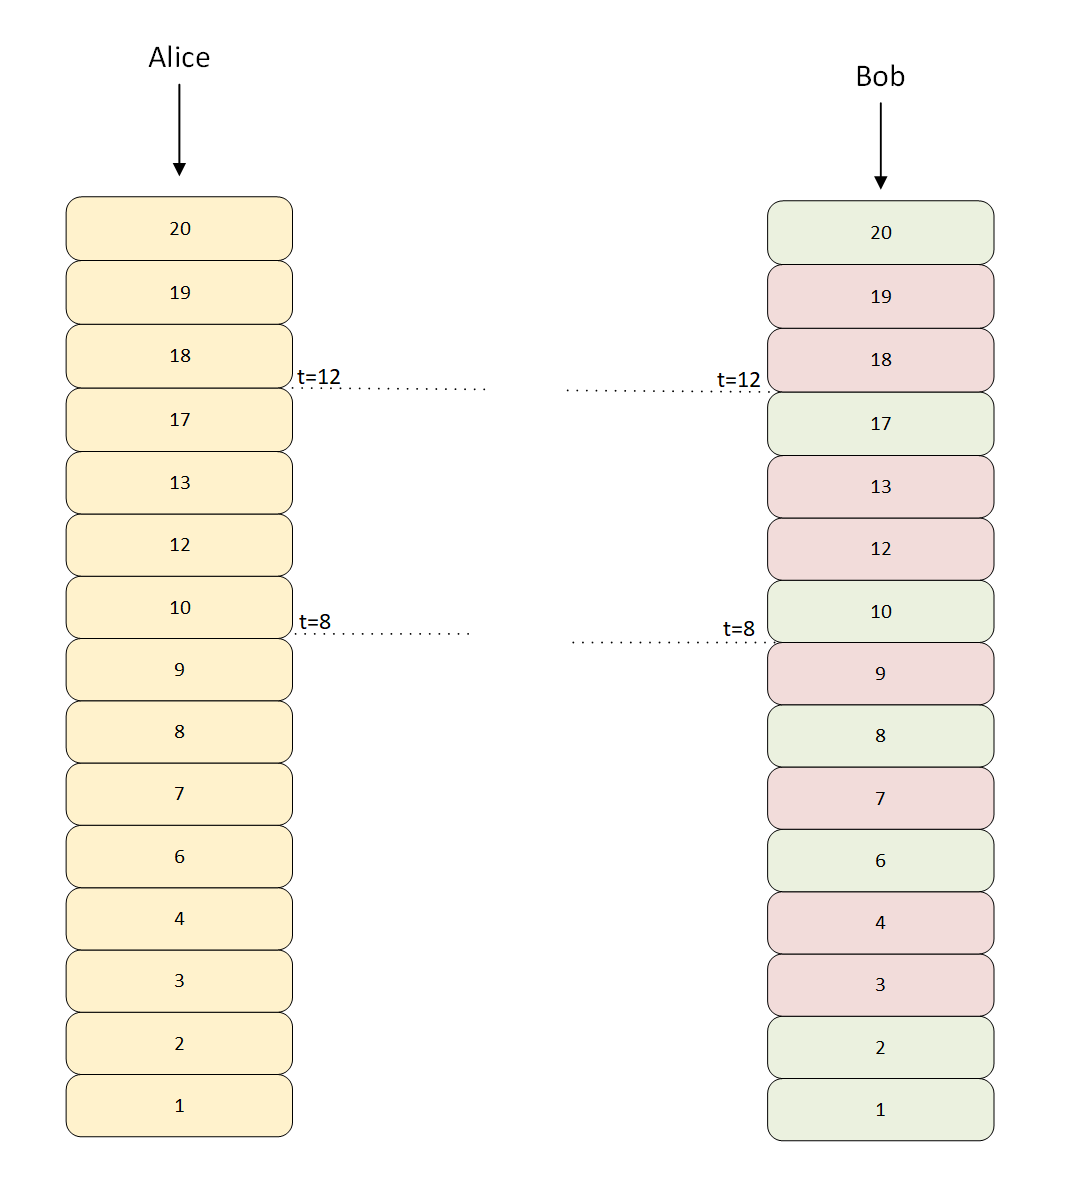
\includegraphics[width=0.7\textwidth, height=8cm]{./figures/alicebobkeys.png}
        	\label{alicebobkeys}
    \end{figure}
Only Bob knows all information about the keys, which correspond to right or random bits. Alice only knows that half are right and half are random bits.

%--------------------------------------------------------------------------------------------------
%------------ SLIDE-------
\mysection{Quantum Oblivious Key Distribution System (QOKD)}
\vspace{2.0cm}
From a QOKD system owe can obtain:\\

\begin{itemize}
  \item Symmetric Secrete Keys.\\
  \item Oblivious Keys.\\
  \item Slightly Oblivious Keys.\\
\end{itemize}

%--------------------------------------------------------------------------------------------------
%------------ SLIDE-------
\mysection{Applications of a QOKD system}
\vspace{2.0cm}

A QOKD system has applicability in two fields:\\

\begin{itemize}
  \item Cryptography.\\
  \item Secure multi-party computation (1-out-of-2 Oblivious Transfer, Nearest Private Query).
\end{itemize}

%------------ SLIDE -------------------------------------------------------------------------------

\mysection{}\large
\vspace{4.0cm}

\begin{center}
    \color{black}\sffamily \noindent \Large
    \br{Quantum Oblivious Key Distribution\\}
    {Protocol detailed}

\end{center}

%--------------------------------------------------------------------------------------------------
%------------ SLIDE -------------------------------------------------------------------------------

\mysection{QOKD - Protocol Detailed}\large
\vspace*{1.0cm}
Alice and Bob build them sets of keys continuously.\\


\begin{description}
  \item[Step 1] Alice and Bob agree with a block length $l$. Lets assume $l=16$. Lets assume Alice generates two sequences with $l$ bits:
      $$S_{A1'} = \{0,0,1,1,1,0,0,1,1,0,0,1,1,1,0,1 \},$$
      $$S_{A2'} = \{1,1,1,0,0,0,0,0,1,1,0,0,1,0,1,1 \}.$$

      where $S_{A1'}$ and $S_{A2'}$ are the sequence of basis and keys with which Alice will encode the photons, respectively.

\end{description}

%--------------------------------------------------------------------------------------------------
%------------ SLIDE -------------------------------------------------------------------------------

\mysection{QOKD - Protocol Detailed}\large
\begin{description}
  \item[Step 2] Alice sends to Bob throughout a quantum channel $l$ encoded photons.
  $$S_{AB} = \{ \uparrow,\uparrow,\nearrow,\searrow,\searrow, \to , \to, \searrow ,\nearrow ,\uparrow ,\to,\searrow,\nearrow,\searrow ,\uparrow ,\nearrow\} $$

  \item[Step 3] Bob also randomly generates $l$ bits to define his measurement basis. Lets assume:
  \begin{align*}
             S_{B1'} & = \{0 \ ,1 \ ,1 \ ,0 \ ,0 \ ,1 \ ,0 \ ,1 \ ,1 \ ,0 \ ,1 \ ,1 \ ,0 \ ,0 \ ,0 \ ,1 \  \} \\
                    & = \{ +,\times,\times,+,+,\times,+,\times, \times,+, \times, \times \,+,+,+,\times \}.
  \end{align*}

   Bob measures $l$ photons and gets a new set,
      $$S_{B2'} = \{1,-,\underline{0},0,-,1,\underline{1},-,1,-,1,0,1,1,\underline{0},1 \}.$$
    where "$-$"\space{ } corresponds to no clicks in Bob's detector, due to attenuation.

\end{description}

%--------------------------------------------------------------------------------------------------
%------------ SLIDE -------------------------------------------------------------------------------

\mysection{QOKD - Protocol Detailed}\large
\vspace*{0.5cm}
\begin{description}
  \item[Step 4] Bob sends a "$-1$"\space{ } or a hash value to Alice for each measurement that he performed. "$-1$"\space{ } corresponds to the measurements when Bob had no clicks.

       $$S_{BH1}=\{{S}_{1},-1,{S}_{2},{S}_{3}, -1,{S}_{4},{S}_{5},-1,{S}_{6},-1,{S}_{7},{S}_{8},{S}_{9},{S}_{10},{S}_{11},{S}_{12} \}.$$

  \item[Step 5] After Alice has received $S_{BH1}$, she sends the basis set which she has used to encode the photons, updated with the information about the no received photons, $$S_{A1'} = \{0,-1,1,1,-1,0,0,-1,1,-1,0,1,1,1,0,1 \}$$.
\end{description}

%--------------------------------------------------------------------------------------------------
%------------ SLIDE -------------------------------------------------------------------------------

\mysection{QOKD - Protocol Detailed}\large
\vspace*{1.0cm}
Due to attenuation, the previous sets are reduced to the length $12$ and they shall be replaced by the following:
\begin{align*}
  S_{A1} & =\{0,1,1,0,0,1,0,1,1,1,0,1 \}, \\
  S_{A2} & =\{1,1,0,0,0,1,0,0,1,0,1,1 \}, \\
  S_{B1} & =\{0,1,0,1,0,1,1,1,0,0,0,1 \}, \\
  S_{B2} & =\{1,\underline{0},0,1,\underline{1},1,1,0,1,1,\underline{0},1 \}
\end{align*}
Note that $S_{B2}$ still has errors.

%--------------------------------------------------------------------------------------------------
%------------ SLIDE -------------------------------------------------------------------------------

\mysection{QOKD - Protocol Detailed}\large
\begin{description}
  \item [Step 6]Bob does the operation $S_{B3}=S_{B1} \oplus S_{A1}$ to verify which photons he measured correctly, $$S_{B3} = \{1,1,0,0,1,1,0,1,0,0,1,1 \}.$$
  Bob has been building two pair of sets, one for the right basis,
  \begin{align*}
    S_{B_{rp}} & = \{1,2,5,6,8,11,12 \}, \\
    S_{B_{rb}} & = \{1,0,1,1,0,0,1 \},
  \end{align*}
  and other pair for photons he measured with the wrong basis and then he just guessed the values,
  \begin{align*}
    S_{B_{wp}} & = \{3,4,7,9,10 \}, \\
    S_{B_{wb}} & = \{0,1,1,1,1 \}.
  \end{align*}


\end{description}

%--------------------------------------------------------------------------------------------------
%------------ SLIDE -------------------------------------------------------------------------------

\mysection{QOKD - Protocol Detailed}\large
In order to test Bob's honesty, Alice estimates the \textit{QBER} of the channel. She must open a minimum number of right positions in order to guarantee a minimum \textit{QBER}.\\
Alice chooses some positions to open and tells Bob which positions she wants to open.\\
Lets assume Alice has verified these pairs using the hash function committed by Bob and concluded that he is being honest. She sends to Bob the \textit{QBER} estimated.

Bob has the previous sets replaced by the following,
  \begin{align*}
    S_{B_{rp}} & = \{1,2,5,6,8 \} \\
    S_{B_{rb}} & = \{1,0,1,1,0 \} \\
    S_{B_{wp}} & = \{3,4,7,9 \} \\
    S_{B_{wb}} & = \{0,1,1,1 \}
  \end{align*}

  %--------------------------------------------------------------------------------------------------
%------------ SLIDE -------------------------------------------------------------------------------

\mysection{QOKD - Protocol Detailed}\large
Since some bits of $S_{B_{rb}}$ were wrongly measured, Bob must apply an error correction algorithm in order to correct the errors due transmission. As there are two sets with wrong and right bits, Bob has to apply a modified version of Cascade Algorithm. He applies the real cascade to $S_{B_{rb}}$ and a fake cascade version to $S_{B_{wb}}$.
After applying the modified version of Cascade Bob gets,

\begin{align*}
S_{B_{rp}} & = \{1,2,5,6,8 \} \\
S_{B_{rb}} & = \{1,1,0,1,0 \} \\
S_{B_{wp}} & = \{3,4,7,9 \} \\
S_{B_{wb}} & = \{0,1,1,0 \}
\end{align*}

Bob has to test Alice's honesty during the cascade algorithm by testing the validity of $QBER$ sent by her.

%--------------------------------------------------------------------------------------------------
%------------ SLIDE -------------------------------------------------------------------------------

\mysection{QOKD - Protocol Detailed}\large
\vspace*{1.0cm}
When Alice sends to Bob a photons set, they are building a set of pairs (array positions and bit values which correspond to measured photons at Bob's side and to the key bit with the photon was encoded at Alice's side).\\

The main goal is to guarantee that Bob has the same number of right and random pairs. In addition, they must know information about $t$.\\


Alice knows that at some tabs there are the same number of right and random bits.

%------------ SLIDE -------------------------------------------------------------------------------

\mysection{}\large
\vspace{4.0cm}

\begin{center}
    \color{black}\sffamily \noindent \Large
    \br{1-out-of-2 Oblivious Transfer\\}
    {Symmetric Oblivious Keys}

\end{center}

%--------------------------------------------------------------------------------------------------
%------------ SLIDE -------------------------------------------------------------------------------

\mysection{1-out-of-2 Oblivious Transfer}\large


\begin{itemize}
    \item {Alice has two messages $m_0$ and $m_1$ and Bob wants to know one of them, $m_b$, without Alice knowing which one, i.e. without Alice knowing $b$, and Alice wants to keep the other message private, i.e. without Bob knowing $m_{\bar{b}}$.}
        Lets assume  $m_{0} = \{0 0 1 1\}$ and $m_{1} = \{0 0 0 1\}$.
    \item Bob defines two sub-sets with size $s=4$ from them sets of keys:
  $$I_{w}=\{3,4,7,9 \},$$
  and $$I_{r}= \{1,2,6,8 \},$$ where $I_{w}$ is the sequence of positions in which Bob was wrong about basis measurement and $I_{r}$ is the sequence of positions in which Bob was right about basis measurement.

\end{itemize}

%--------------------------------------------------------------------------------------------------
%------------ SLIDE--------------------------------------------------------------------------------
\mysection{1-out-of-2 Oblivious Transfer}\large

\begin{itemize}
  \item Lets assume Bob wants to know $m_{0}$.
  He sends to Alice the set $S=\{I_{r}, I{w}\}.$
  \item Alice defines two encryption keys $K_{0}$ and $K_{1}$ using the values in positions defined by Bob in the set sent by him. Lets assume, $$K_{0}=\{1,1,1,0\}$$ $$K_{1}=\{0,0,0,1\}.$$ Alice does the following operations:
   $$m = \{m_{0}\oplus K_{0}, m_{1} \oplus K_{1} \}.$$
  \item Alice sends to Bob $$m=\{1,1,0,1,0,0,0,0\}.$$
\end{itemize}



%--------------------------------------------------------------------------------------------------
%------------ SLIDE--------------------------------------------------------------------------------
\mysection{1-out-of-2 Oblivious Transfer}\large

\begin{itemize}

  \item Bob uses values from $S_{B1\prime}$ at positions given by $S$ and does the decrypted operation.

   \begin{table}[hbt]
        \centering
        \begin{tabular}{c|c c c c c c c c}
         $m$ & 1 & 1 & 0 & 1 & 0 & 0 & 0 & 0 \\
             & 1 & 1 & 1 & 0 & 0 & 1 & 1 & 0 \\ \hline
         $\oplus$ & 0 & 0 & 1 & 1 & 0 & 1 & 1 & 0 \\
        \end{tabular}
        \end{table}
    The first four bits corresponds to message 0 and he received $\{0,0,1,1\}$, which is the right message $m_{0}$ and $\{0,1,1,0\}$ which is a wrong message for $m_{1}$.
\end{itemize}

%------------ SLIDE -------------------------------------------------------------------------------

\mysection{}\large
\vspace{4.0cm}

\begin{center}
    \color{black}\sffamily \noindent \Large
    \br{Nearest Private Query\\}
    {Asymmetric Oblivious Keys}

\end{center}
%--------------------------------------------------------------------------------------------------
%------------ SLIDE--------------------------------------------------------------------------------
\mysection{Nearest Private Query}\large

\begin{itemize}
  \item Assuming two parties, a user (Bob) and a data owner (Alice).\\
  \item Bob has an input secrete parameter $x$. Lets assume $x=8$.\\
  \item Alice has a private data set, $A=\{ 1,2,3,6,7,10,11,14\}$.\\
  \item Bob wants to know which element ($x_{i}$) is the closest to $x$ in Alice data set $A$, without revealing his secrete $x$.\\
  \item Alice cannot know anything about the secrete information $x$, and Bob cannot know secrete information about the private data set $A$ except the near parameter, $x_{i}$.

\end{itemize}

%--------------------------------------------------------------------------------------------------
%------------ SLIDE--------------------------------------------------------------------------------
\mysection{Nearest Private Query}\large

\begin{itemize}
  \item Alice generates a new set with $N=2^{n}$ elements, $D(j)$ for $j=0,1,...N-1$ in which $D(j)=x_{l}$ being $x(l)$ the closest element to $j$ in $A$. $n$ is the number of bits that Alice needs to represent each element of her data set.\\
  \begin{table}[hbt]
        \centering
        \begin{tabular}{c|c|c|c|c|c|c|c|c|c|c|c|c|c|c|c|c}
        \textbf{$j$}    & 0 & 1 & 2 & 3 & 4 & 5 & 6 & 7 & 8 & 9  & 10 & 11 & 12 & 13 & 14 & 15 \\ \hline
        \textbf{$D(j)$} & 1 & 1 & 2 & 3 & 3 & 6 & 6 & 7 & 7 & 10 & 10 & 11 & 11 & 14 & 14 & 14 \\ \hline
                        & 0 & 0 & 0 & 0 & 0 & 0 & 0 & 0 & 0 & 1  & 1  & 1  & 1  & 1  & 1  & 1  \\
                        & 0 & 0 & 0 & 0 & 0 & 1 & 1 & 1 & 1 & 0  & 0  & 0  & 0  & 1  & 1  & 1  \\
                        & 0 & 0 & 1 & 1 & 1 & 1 & 1 & 1 & 1 & 1  & 1  & 1  & 1  & 1  & 1  & 1  \\
                        & 1 & 1 & 0 & 1 & 1 & 0 & 0 & 1 & 1 & 0  & 0  & 1  & 1  & 0  & 0  & 0
        \end{tabular}
  \end{table}



\end{itemize}

%--------------------------------------------------------------------------------------------------
%------------ SLIDE--------------------------------------------------------------------------------
\mysection{Nearest Private Query}\large
\begin{itemize}
  \item Bob and Alice have a set of keys $K_{i}^*$ and $K_{i}$, respectively, with $64$ elements where $60$ are bits resulted from wrong basis measurement and $4$ resulted from correct basis measurement. This allows Alice to know that Bob is being honest.\\
  \item Bob sends to Alice the set $S$ with wrong bits positions except at $j=8$.\\
  \item Alice gets the closest number to $x=8$ which is $7$ and she remains know nothing about the other elements.
\end{itemize}

%--------------------------------------------------------------------------------------------------
%------------ SLIDE-------
\mysection{Simulation Setup}\large

\begin{figure}[hbt]
    	\centering
    	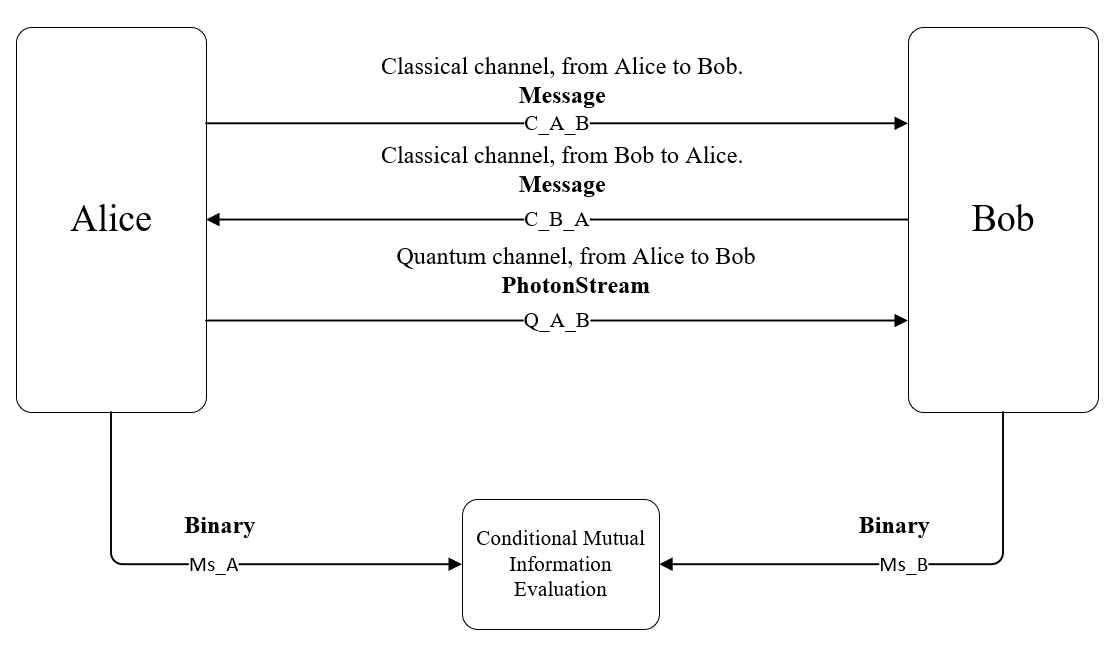
\includegraphics[width=1\textwidth, height=10cm]{./figures/Simulation_diagram_top.png}
        	\label{alicebobkeys}
    \end{figure}

%--------------------------------------------------------------------------------------------------
%------------ SLIDE-------
\mysection{Simulation Setup - Alice}\large

\begin{figure}[hbt]
    	\centering
    	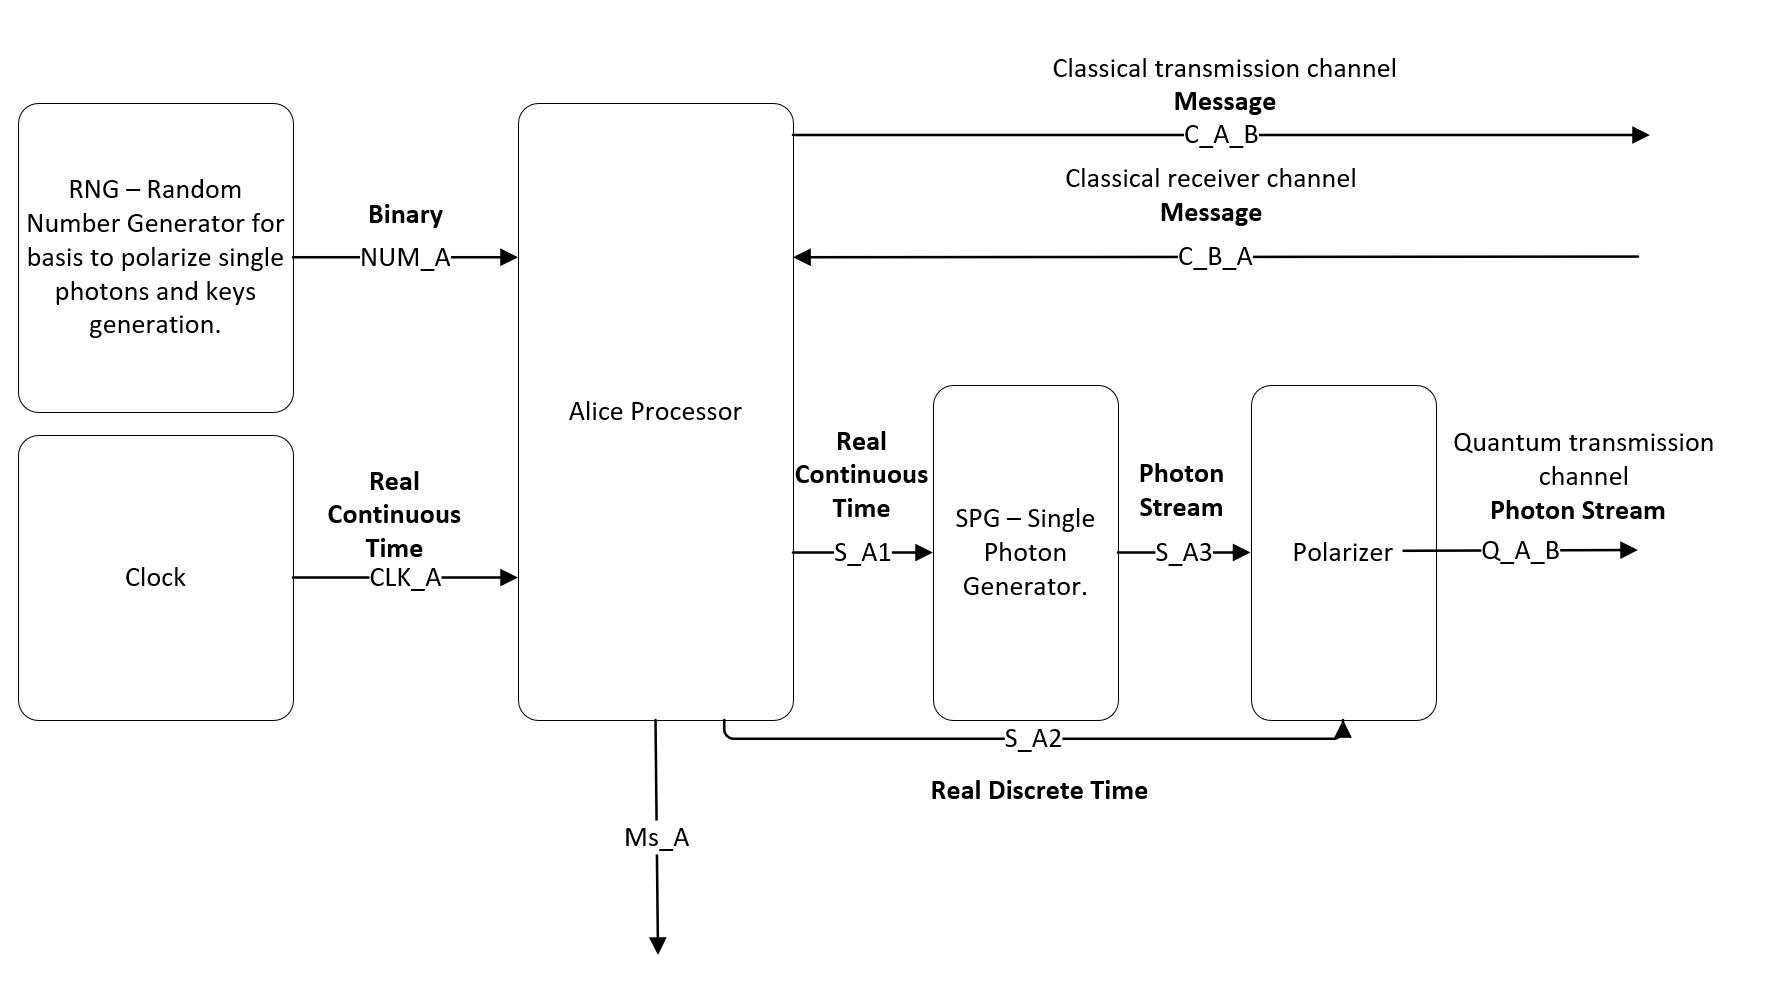
\includegraphics[width=1\textwidth, height=10cm]{./figures/Simulation_Alice.png}
        	\label{alicebobkeys}
    \end{figure}

%--------------------------------------------------------------------------------------------------
%------------ SLIDE-------
\mysection{Simulation Setup - Bob}\large

\begin{figure}[hbt]
    	\centering
    	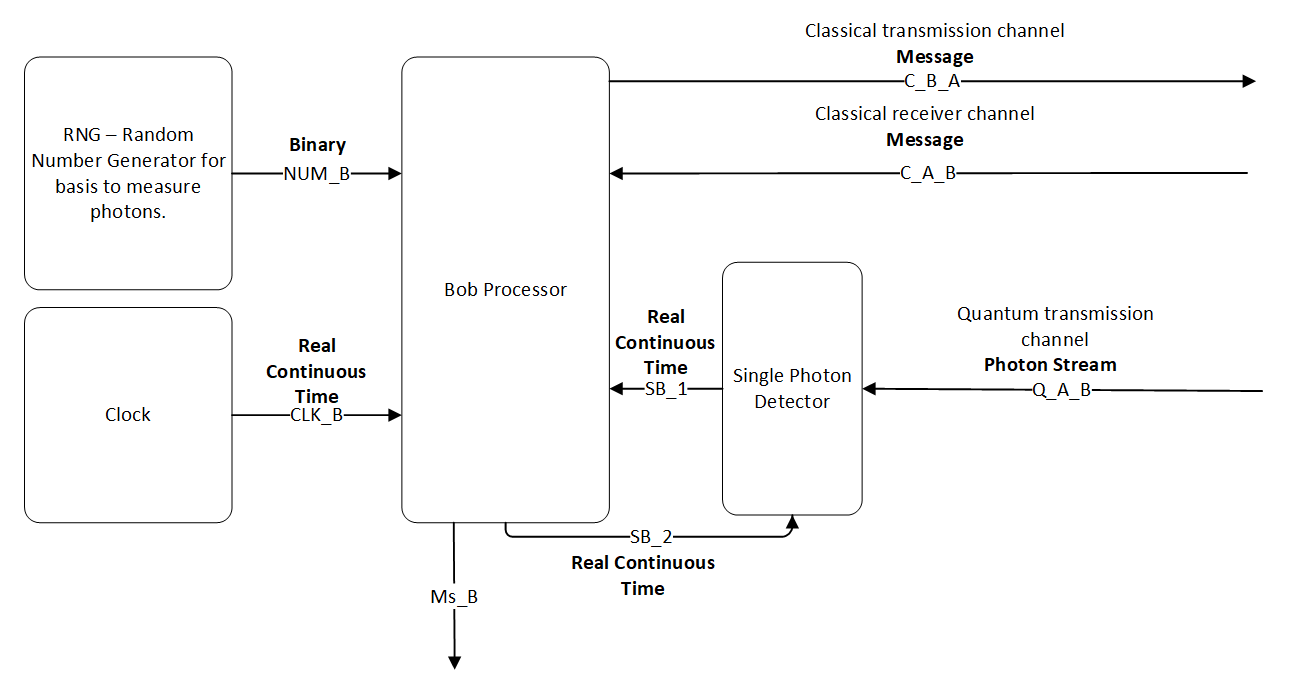
\includegraphics[width=1\textwidth, height=9cm]{./figures/Simulation_Bob.png}
        	\label{alicebobkeys}
    \end{figure}


%--------------------------------------------------------------------------------------------------
%------------ SLIDE-------
\mysection{Experimental Setup}\large

\begin{figure}[hbt]
    	\centering
    	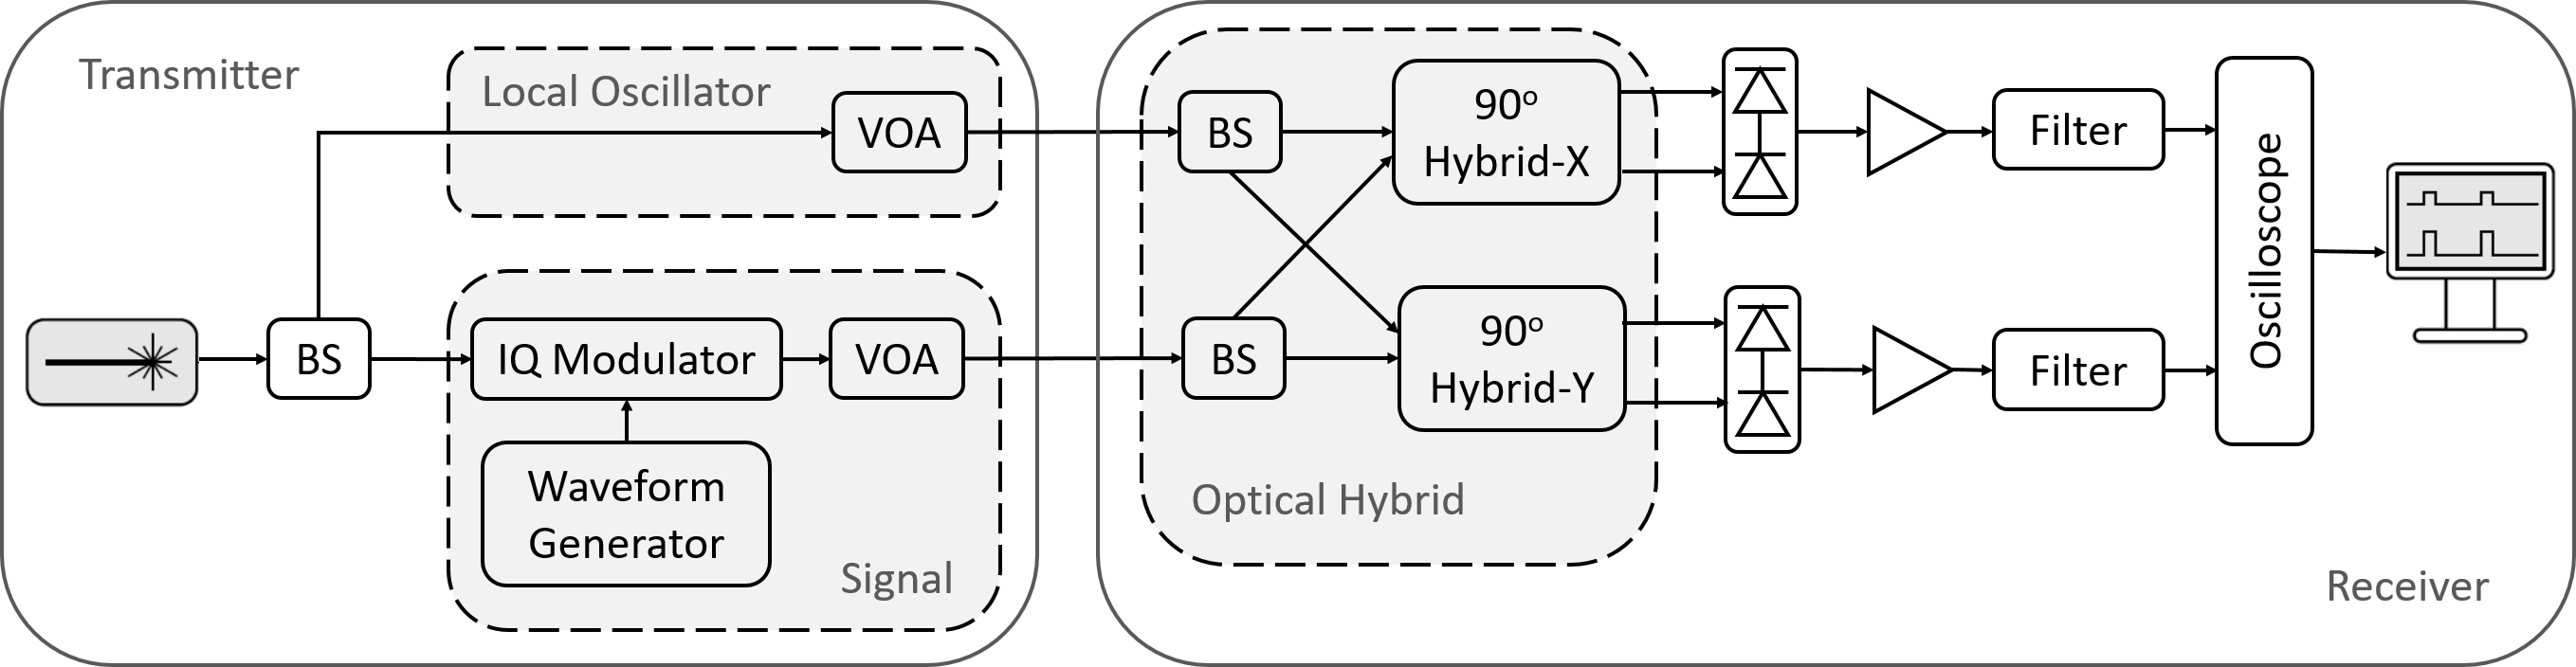
\includegraphics[width=0.9\textwidth, height=9cm]{./figures/experimental_setup.png}
        	\label{alicebobkeys}
    \end{figure}


%-------------------------------------------------------------------
%------------ SLIDE ------------------------------------------------
\mysection{} \sffamily
\vspace{-10mm}
\large\centerline{E-mail: marianaferreiraramos@ua.pt}


\end{document}
